\chapter{La misurazione in psicologia}
\label{chapter:misurazione} 


%I ricercatori cercano di rispondere alle domande della ricerca usando metodologie rigorose e osservazioni accurate. 
Le osservazioni empiriche -- osservazioni sul campo, sondaggi o risultati di esperimenti -- forniscono il materiale che viene utilizzato in un'indagine statistica e sono chiamate \emph{dati}. 
%La statistica ci fornisce un insieme di strumenti utili per raccogliere, analizzare e trarre conclusioni dai dati. 
%L'analisi dei dati è una componente dell'indagine scientifica i cui scopi sono:
%\begin{enumerate}
%\item identificare una domanda o un problema;
%\item raccogliere dati rilevanti sull'argomento;
%\item analizzare i dati;
%\item formare una conclusione.
%\end{enumerate}
%La statistica si concentra sulle fasi 2-4. 
%Cioè, si pone le seguenti domande: qual è il modo migliore per raccogliere i dati? Come essi dovrebbero essere analizzati? 
%E cosa possiamo dedurre dall'analisi?
Quando parliamo di dati dobbiamo chiederci: in che misura i dati che sono stati raccolti sono in grado di rappresentare in maniera veritiera le caratteristiche del fenomeno  esaminato?
C'è un'intera disciplina che cerca di rispondere alla domanda precedente: la \enquote{teoria della misurazione}.
Senza entrare nei dettagli, il presente capitolo intende fornire un'introduzione generale alle tematiche della misurazione in psicologia.


\section{Le scale di misura}

%Secondo Stevens (1947), esistono quattro modi in cui le modalità di una variabile sono in grado di rappresentare le variazioni del fenomeno considerato:
%\begin{description}
%\item [Uguaglianza:] è ammessa la sola relazione di equivalenza tra le misure delle unità statistiche. 
%In una classe di oggetti possiamo stabilire solo se due di essi sono uguali o diversi. 
%\item [Ordine:] I numeri che vengono assegnati alle modalità non corrispondono all'intensità della proprietà misurata: essi rappresentano soltanto la relazione d'ordine (``più grande di'') tra le modalità. Possiamo stabilire che l'intensità di una proprietà di un oggetto è maggiore di quella di un altro oggetto, ma non sappiamo di quanto.
%\item [Intervallo unitario:] diventa possibile misurare le distanze tra le coppie di unità statistiche nei termini di un intervallo costante, chiamato unità di misura, a cui viene attribuito il valore ``1''.
%\item [Zero assoluto:] la scala ha un vero punto zero al di sotto del quale non esistono valori. Ad esempio, non è possibile che il peso di una persona sia negativo.
%\end{description}

I risultati delle misurazioni, ovvero le variabili, devono avere almeno due valori possibili (altrimenti sarebbero delle costanti).
È importante notare che le modalità delle variabili sono in grado di descrivere l'intensità del fenomeno misurato con livelli diversi di precisione. 
La capacità delle variabili di ``catturare'' in forma numerica le proprietà del fenomeno che esse rappresentano viene descritta dalla teoria delle scale di misura di \citet{stevens46}. 
Secondo tale teoria, possiamo distinguere quattro scale di misura aventi proprietà diverse (Figura~\ref{fig:Stevens}): le scale nominali (\emph{nominal scales}), ordinali (\emph{ordinal scales}), a intervalli (\emph{interval scales}), di rapporti (\emph{ratio scales}).

\begin{figure}
% \centering
% \floatbox {figure}
\begin{tikzpicture}[scale=0.9,text height=1.5ex,text depth=.25ex]
  \node (h) at (2.3, 0) {};
  \node (v) at (0,0.8) {};
  \node (Nominal) at (1, 2) {Nominale};
  \node (Ordinal) at ($(Nominal)+(h)$) {Ordinale};
  \node (Interval) at ($(Nominal)+2*(h)$) {Intervalli};
  \node (Ratio) at ($(Nominal)+3*(h)$) {Rapporti};
  \node (Equality) at ($(Nominal)-3*(v)$) {$=\ne$};
  \node (LessMore) at ($(Ordinal)-3*(v)$) {$<>$};
  \node (PlusMinus) at ($(Interval)-3*(v)$) {$+-$};
  \node (MultiplyDivide) at ($(Ratio)-3*(v)$) {$\times\div$};
  \node [text width=2cm,text centered] (Mutual) at ($(Nominal)-1.5*(v)$) {Categorie distinte};
  \node [text width=2cm,text centered] (Order) at ($(Ordinal)-1.5*(v)$) {Categorie ordinate};
  \node [text width=2cm,text centered] (Distance) at ($(Interval)-1.5*(v)$) {Distanze costanti};
  \node [text width=2cm,text centered] (Magnitude) at ($(Ratio)-1.5*(v)$) {Zero assoluto};
  \node [color=black] (Level) at ($(Nominal)-1.2*(h)$) {\textbf{Livello}};
  \node [text width=2cm,text centered, color=black] (Feature) at ($(Level)-1.5*(v)$) {\textbf{Caratteristiche}}; 
  \node [color=black] (Operation) at ($(Level)-3*(v)$) {\textbf{Operazioni}}; 
\draw[decoration={brace,amplitude=3mm}, decorate] (Nominal.north) -- (Ordinal.north) node[midway,above=3mm] (Categorical) {Categoriale};
  \draw[decoration={brace,amplitude=3mm}, decorate] (Interval.north) -- (Ratio.north) node[midway,above=3mm] (Quantitative) {Quantitativa};
    \draw[decoration={brace,amplitude=3mm}, decorate] (Categorical.north) -- (Quantitative.north) node[midway,above=3mm] (Variable) {Variabile};
\end{tikzpicture}
\caption{I quattro livelli di scala secondo \citet{stevens46}.}
\label{fig:Stevens}
\end{figure}

\subsection{Scala nominale}

La scala nominale raggruppa i dati in categorie qualitative \emph{mutuamente esclusive} (cioè nessun dato si può collocare in più di una categoria). 

Esiste la sola relazione di equivalenza tra le misure delle u.s., cioè nella scala nominale gli elementi del campione appartenenti a classi diverse sono differenti, mentre tutti quelli della stessa classe sono tra loro equivalenti: $x_i = x_j$ oppure $x_i \neq x_j$. È ammessa l'operazione del conteggio delle u.s. presenti in ogni categoria e il conteggio delle classi di equivalenze, dunque la descrizione dei dati avviene tramite le frequenze assolute e le frequenze relative. 

A partire da una scala nominale è possibile costruire altre scale equivalenti trasformando i valori della scala di partenza in modo tale da cambiare i nomi delle modalità ma lasciando però inalterata la suddivisione u.s. nelle medesime classi di equivalenza. Questo significa che prendendo una variabile misurata su scala nominale e cambiando i nomi delle sue categorie otteniamo una nuova variabile esattamente corrispondente alla prima. 

%\begin{oss}
%Anche nel caso del livello più basso della misurazione (scale nominali), però nel mondo empirico sono poche le variabili nominali che hanno esattamente le proprietà descritte sopra. 
%Per esempio, si consideri la diagnosi di disabilità intellettiva, ciò che è stato storicamente chiamato ``ritardo mentale''. 
%Potremmo avere solo due categorie nel nostro schema di codifica (Disabilità intellettiva: Sì o No) ma è ampiamente riconosciuto che la condizione viene espressa in gradi (es., ``nulla'' ``borderline'', ``lieve'', `` moderato'', ``grave'' e ``estremo''). 
%Pertanto, il costrutto di disabilità intellettiva non è nemmeno concettualmente a livello di scala nominale; è invece un continuum che è stato diviso in un certo punto per convenienza, in un modo arbitrario. 
%Distinguere tra una variabile dicotomica che è nominale per natura e una che ha un (implicito) continuum sottostante è importante perché alcuni indici statistici possono essere calcolati solo nel caso di quest'ultimo tipo di variabile (ad esempio, il coefficiente di correlazione tetracorica).
%
%Cosa succede se le categorie della scala nominale non si escludono a vicenda? 
%Ad esempio, supponiamo di avere una variabile in cui le persone possono essere classificate come affette da sindrome di Down o sindrome di Klinefelter (XXY). 
%Ovviamente, questa è una falsa dicotomia. 
%La maggior parte delle persone non ha nessuna delle due condizioni. 
%Bene, possiamo espandere la variabile nominale in tre categorie: sindrome di Down, sindrome di Klinefelter e nessuna delle due. 
%Cosa succede se una persona ha sia la sindrome di Down che la sindrome di Klinefelter? 
%Ok, aggiungiamo una quarta categoria: entrambe. 
%Questo approccio combinatorio può essere perseguito per alcuni scopi (ad esempio, il sistema dei gruppi sanguigni ABO), ma per molte variabili diventa rapidamente ingestibile. 
%Se volessimo descrivere tutte le anomalie cromosomiche con una singola variabile nominale, il numero di combinazioni aumenterebbe esponenzialmente con ogni nuova categoria aggiunta. 
%Questo potrebbe andar bene se fosse molto raro avere due o più anomalie cromosomiche. 
%Se, tuttavia, le categorie non si escludono a vicenda e le combinazioni sono abbastanza comuni, in genere è più semplice descrivere il fenomeno usando due o più variabili nominali (sindrome di Down: sì o no; sindrome di Klinefelter: sì o no; sindrome di Edwards: sì o no e così via). 
%Si noti che alcune false dicotomie sono usate così comunemente  che le persone sanno cosa intendiamo quando le usiamo, anche se tali dicotomie sono incomplete (ad esempio, di sinistra vs. di destra) o potenzialmente insensibili a persone che non si adattano perfettamente a nessuna delle categorie tipiche (ad esempio, maschio vs. femmina).
%\end{oss}


\subsection{Scala ordinale}

La scala ordinale conserva la proprietà della scala nominale di classificare ciascun dato all'interno di una sola categoria, ma alla relazione di equivalenza tra elementi di una stessa classe aggiunge la relazione di ordinamento tra le varie classi di equivalenza.  
%I numeri che vengono assegnati alle modalità non corrispondono all'intensità della proprietà misurata: essi rappresentano soltanto la relazione d'ordine  (``più grande di'') tra le modalità. 
Essendo basata su una relazione d'ordine, una scala ordinale descrive soltanto l'ordine di rango tra le modalità, ma non dà alcuna informazione su quanto una modalità sia più grande di un'altra. 
Non ci dice, per esempio, se la distanza tra le modalità $a$ e $b$ sia uguale, maggiore o minore della distanza tra le modalità $b$ e $c$. 

Un esempio classico di scala ordinale è quello della scala Mohs per la determinazione della durezza dei minerali. 
Per stabilire la durezza dei minerali si usa il criterio empirico della scalfittura.
Vengono stabiliti livelli di durezza crescente da 1 a 10 con riferimento a dieci minerali: talco, gesso, calcite, fluorite, apatite, ortoclasio, quarzo, topazio, corindone e diamante. 
Un minerale appartenente ad uno di questi livelli se scalfisce quello di livello inferiore ed è scalfito da quello di livello superiore. 

%\begin{oss}
%La maggior parte delle misurazioni nella valutazione psicologica coinvolge scale ordinali, anche se in molti casi le scale ordinali vengono confuse con altri tipi di scale. 
%I questionari che usano le scale di tipo Likert sono chiaramente ordinali (Figura~\ref{fig:Likert}). 
%Anche se gli item vero / falso nei questionari potrebbero sembrare a livello di scala nominale, di solito sono ordinali perché la risposta indica se una persona possiede in grado maggiore o minore un dato attributo; cioè, \emph{più} e \emph{meno} sono concetti intrinsecamente ordinali. 
%Allo stesso modo, gli item dei test di abilità sono anch'essi ordinali, anche se \emph{corretto} o \emph{incorretto} potrebbero sembrare categorie nominali. 
%I test di abilità sono progettati in modo tale che una risposta corretta indichi un grado di abilità maggiore di una risposta errata. 
%La natura ordinale degli item dei test di abilità è particolarmente chiara nei casi in cui è consentito il credito parziale.
% 
%\begin{figure}
%\centering
%\begin{tikzpicture} [font=\normalsize]
%\node [align=center,text width=3cm] (sd)  {\textbf{Per niente d'accordo}};
%\node [align=center,text width=3cm,above=of sd]  (d) {\textbf{Disaccordo}};
%\node [align=center,text width=3cm,above=of d]  (n) {\textbf{Indeciso}}; 
%\node [align=center,text width=3cm,above=of n] (a)  {\textbf{D'accordo}};
%\node [align=center,text width=3cm,above=of a] (sa) {\textbf{Molto d'accordo}};
%\draw [decoration={brace,amplitude=3mm}, decorate] (d.east) -- (sd.east) node[midway, rotate=-90,align=center,yshift=2em]{Distanza?};
%\draw [decoration={brace,amplitude=3mm}, decorate] (d.west) -- (n.west) node[midway, rotate=90,align=center,yshift=2em]{Distanza?};
%\draw [decoration={brace,amplitude=3mm}, decorate] (a.east) -- (n.east) node[midway, rotate=-90,align=center,yshift=2em]{Distanza?};
%\draw [decoration={brace,amplitude=3mm}, decorate] (a.west) -- (sa.west) node[midway, rotate=90,align=center,yshift=2em]{Distanza?};
%\draw (sd.north) -- (d.south);
%\draw (d.north) -- (n.south);
%\draw (n.north) -- (a.south);
%\draw (a.north) -- (sa.south);
%\end{tikzpicture}
%\caption{In una scala Likert le distanze tra le categorie non sono definite.}
%\label{fig:Likert}
%\end{figure}
%
%Le operazioni algebriche ammesse sulle misure a livello di scala ordinale sono analoghe a quelle consentite per le scale nominali. 
%
%A partire da una scala ordinale è possibile costruire altre scale equivalenti trasformando i valori della scala di partenza per mezzo di qualunque trasformazione che preservi l'ordinamento tra le modalità. 
%\end{oss}


%----------------------------------------------------------------------------
\subsection{Scala ad intervalli}

La scala ad intervalli include le proprietà di quella nominale e di quella ordinale, e in più consente di misurare le distanze tra le coppie di u.s. nei termini di un intervallo costante, chiamato \emph{unità di misura}, a cui viene attribuito il valore ``1''.  La posizione dell'origine della scala, cioè il punto zero, è scelta arbitrariamente, nel senso che non indica l'assenza della quantità che si sta misurando. Avendo uno zero arbitrario, questa scala di misura consente valori negativi. Lo zero, infatti, \emph{non} viene attribuito all'u.s. in cui la proprietà misurata risulta assente.
 
La scala a intervalli equivalenti ci consente di effettuare operazioni algebriche basate sulla differenza tra i numeri associati ai diversi punti della scala, operazioni algebriche non era possibile eseguire nel caso di misure a livello di scala ordinale o nominale. Il limite della scala ad intervalli è  quello di non consentire il calcolo del rapporto tra coppie di misure. Possiamo dire, per esempio, che la distanza tra  $a$ e $b$ è la metà della distanza tra $c$ e $d$. Oppure che la distanza tra $a$ e $b$ è uguale alla distanza tra $c$ e $d$. Non possiamo dire, però, che  $a$ possiede la proprietà misurata in quantità doppia rispetto  $b$. Non possiamo cioè stabilire dei rapporti diretti tra le misure ottenute. Solo per le \emph{differenze} tra le modalità sono dunque permesse tutte le operazioni aritmetiche: le differenze  possono essere tra loro sommate, elevate a potenza oppure divise, determinando così le quantità che stanno alla base della statistica inferenziale. 
 
Nelle scale ad intervalli equivalenti, l'unità di misura è arbitraria, ovvero può essere cambiata attraverso una dilatazione, operazione che consiste nel moltiplicare tutti i valori della scala per una costante positiva.
Poiché l'aggiunta di una costante non altera le differenze tra i valori della scala, è anche ammessa la traslazione, operazione che consiste nel sommare una costante a tutti i valori della scala. 
Essendo la scala invariate rispetto alla traslazione e alla dilatazione, le trasformazioni ammissibili sono le \emph{trasformazioni lineari}:
\[
y' = a + by, \quad b > 0.
\]

Esempio di scala ad intervalli è la temperatura misurata in gradi Celsius o Fahrenheit, ma non Kelvin. 
Come per la scala nominale, è possibile stabilire se due modalità sono uguali o diverse: 30$^\circ$C $\neq$ 20$^\circ$C. 
Come per la scala ordinale è possibile mettere due modalità in una relazione d'ordine: 30$^\circ$C $>$ 20$^\circ$C. 
In aggiunta ai casi precedenti, però, è possibile definire una unità di misura per cui è possibile dire che tra 30$^\circ$C e 20$^\circ$C c'è una differenza di 30$^\circ$ - 20$^\circ$ = 10$^\circ$C. 
I valori di temperatura, oltre a poter essere ordinati secondo l'intensità del fenomeno, godono della proprietà che le differenze tra loro sono direttamente confrontabili e quantificabili.  

Il limite della scala ad intervalli è quello di non consentire il calcolo del rapporto tra coppie di misure. 
Ad esempio, una temperatura di 80$^\circ$C non è il doppio di una di 40$^\circ$C.  
Se infatti esprimiamo le stesse temperature nei termini della scala Fahrenheit, allora i due valori non saranno in rapporto di 1 a 2 tra loro. Infatti, 20$^\circ$C = 68$^\circ$F e 40$^\circ$C = 104$^\circ$F. Questo significa che la relazione ``il doppio di'' che avevamo individuato in precedenza si applicava ai numeri della scala centigrada, ma non alla proprietà misurata (cioè la temperatura). 
La decisione di che scala usare (Centigrada vs. Fahrenheit) è arbitraria.  
Ma questa arbitrarietà non deve influenzare le inferenze che traiamo dai dati. 
Queste inferenze, infatti, devono dirci qualcosa a proposito della realtà empirica e non possono in nessun modo essere condizionate dalle nostre scelte arbitrarie che ci portano a scegliere la scala Centigrada piuttosto che quella Fahrenheit.

L'aspetto che rimane invariante a seguito di una trasformazione lineare è l'uguaglianza dei rapporti fra intervalli. Consideriamo, ad esempio, tre temperature: 20$^\circ$C = 68$^\circ$F; 15$^\circ$C = 59$^\circ$F; 10$^\circ$C = 50$^\circ$F. È facile rendersi conto del fatto che i rapporti fra intervalli restano costanti indipendentemente dall'unità di misura che è stata scelta:
\[
\frac{20^\circ C - 10^\circ C}{20^\circ C - 15^\circ C} = 
\frac{68^\circ F - 50^\circ F}{68^\circ F-59^\circ F} = 2.
\]

%\begin{oss}
%Non è sempre facile distinguere tra una scala a intervalli e una scala ordinale. 
%I terapeuti a volte chiedono ai clienti di valutare il loro disagio ``su una scala da 0 a 10.'' 
%Probabilmente, nella mente del terapeuta, la distanza tra ogni punto della scala è uguale. 
%Nella mente del cliente, tuttavia, le cose potrebbero non stare così. 
%Nella Figura~\ref{fig:suds} un ipotetico cliente pensa che la distanza tra 9 e 10 sia maggiore della distanza tra 0 e 1. 
%
%\begin{figure} 
%\centering
%\begin{tikzpicture}[scale=1]
%    \definecolor{firebrick2}{RGB}{205,38,38};
%    \definecolor{royalblue2}{RGB}{67,110,238};
%   \pgfmathtruncatemacro{\T}{10}
%   \tikzstyle{every node}=[draw=none,shape=circle,ball color=royalblue2,minimum size=5.5mm];
%   \foreach \n in {0,...,\T} 
%      \node (\n) at (0,\n) {\footnotesize{\n}};
%   \foreach \n [remember=\n as \lastn (initially 0)] in {0,...,\T} 
%      \draw (\lastn) -- (\n);
%   \tikzstyle{every node}=[draw=none,shape=circle,ball color=firebrick2,minimum size=5.5mm];
%\def\myarray{{0,0.63,1.45,2.36,3.33,4.35,5.42,6.52,7.65,8.81,11}};
%   \foreach \x [count=\xi] in {0,...,10} 
%      \node (\x) at (1,\myarray[\x]) {\footnotesize{\x}};
%   \foreach \x [remember=\x as \lastx (initially 0)] in {0,...,\T} 
%      \draw (\lastx) -- (\x);
%   \tikzstyle{every node}=[rotate=-90];
%\node at (-0.8,5) {\textbf{\small{Scala ipotizzata (intervalli costanti)}}};
%\node at (1.8,5) {\textbf{\small{Scala effettivamente usata da un paziente (intervalli non costanti)}}};
%\end{tikzpicture} 
%\caption{Le unità soggettive di disagio psicologico potrebbero non essere separate da distanze costanti.}
%\label{fig:suds}
%\end{figure} 
%
%Ci si può chiedere se una misurazione di proprietà soggettive possa mai essere rappresentata ad un livello di scala ad intervalli. 
%La maggior parte degli strumenti utilizzati nella valutazione psicologica fa uso di scale ordinali e le trasforma in modo tale da trattarle come se fossero scale a intervalli. 
%Tale approccio è difendibile? 
%Sì, una difesa è possibile: gli psicologi sono consapevoli di questa difficoltà e, all'interno di certi limiti, è stato affermato che una tale \emph{approssimazione} non produce distorsioni troppo grandi. 
%Altri psicologi, invece, non sono convinti che un tale modo di procedere sia sensato.
%In generale, come atto di fede, la maggior parte degli psicologi \emph{assume} che la maggior parte delle scale utilizzate nella valutazione psicologica (misure di abilità, tratti della personalità, atteggiamenti, interessi, motivazione e così via) siano abbastanza vicine alle scale intervallate da poter essere trattate come tali.
%In alcuni casi, tale fede può essere mal riposta, ma dove esattamente ciò accade è difficile da stabilire. 
%Sembra dunque sensato cercare di bilanciare l'atto di fede descritto sopra con una moderata cautela.
%\end{oss}

\subsection{Scala di rapporti}

Nella scala a rapporti equivalenti la posizione dello zero non è arbitraria, ma corrisponde all'elemento dotato di intensità nulla rispetto alla proprietà misurata. Una scala a rapporti equivalenti si costruisce associando il numero 0 all'elemento con intensità nulla; viene  poi scelta un'unità di misura $u$ e, ad ogni elemento, si assegna un numero $a$ definito come:
\[
a = \frac{d}{u}
\]
dove $d$ rappresenta la distanza dall'origine. Alle u.s.  vengono dunque assegnati dei numeri tali per cui le differenze e i rapporti tra i numeri  riflettono le differenze e i rapporti tra le intensità della proprietà misurata.

Operazioni aritmetiche sono  possibili non solo sulle differenze tra i valori della scala (come per la scala a intervalli equivalenti), ma anche sui valori stessi della scala. L'unica arbitrarietà riguarda l'unità di misura che si utilizza. L'unità di misura può cambiare, ma qualsiasi unità di misura si scelga, lo zero deve sempre indicare l'intensità nulla della proprietà considerata.

Le trasformazioni ammissibili a questo livello di scala sono dette trasformazioni di similarità:
\[
    y' = by, \quad b > 0.
\]
A questo livello di scala, a seguito delle trasformazioni ammissibili, rimangono invariati anche i rapporti:
\[
    \frac{y_i}{y_j} = \frac{y'_i}{y'_j}.
\]


%\begin{oss}
%Nella valutazione psicologica sono comunemente usate delle autentiche scale di rapporti. 
%Ogni qualvolta che si conta il numero di occorrenze di qualcosa (ad esempio, quando si calcola la frequenza con cui si verifica un comportamento in un'osservazione diretta), otteniamo una misura a livello di scala di rapporti. 
%Tuttavia, ci sono delle complicazioni. 
%Se osservo quante volte un bambino parla in classe quando non dovrebbe e uso tale frequenza come indice di impulsività, non ho più una scala di rapporti. 
%Perché? 
%Il numero di occorrenze è certamente una variabile a livello di rapporti perché zero occorrenze corrispondono all'assenza del fenomeno. 
%Tuttavia, se uso il numero di occorrenze come una variabile che codifica l'impulsività, allora l'evento che corrisponde a zero occorrenze nelle quali un bambino parla quando non dovrebbe probabilmente non indicano un'assenza di impulsività. 
%Nella migliore delle ipotesi il valore zero indica un basso livello di impulsività. 
%Questo stesso problema esiste per la misurazione dei tempi di reazione. 
%Il tempo di reazione sembra essere a livello di rapporti poiché un tempo di reazione di zero significa che non è trascorso alcun tempo tra la presentazione dello stimolo e la risposta. 
%Tuttavia, i tempi di reazione usati nelle applicazioni cliniche sono spesso utilizzati per codificare tratti psicologici quali la disattenzione, i quali sono costrutti a livello di intervalli. 
%Perché è sensato concepire i tratti psicologici quali le abilità cognitive, i tratti della personalità e così via, come costrutti a livello di scala ad intervalli? 
%Perché non sappiamo ancora come stabilire a cosa corrisponda, per esempio, il livello zero dell'intelligenza o il livello zero dell'estroversione. 
%\end{oss}


%-=-=-=-=-=-=-=-=-=-=-=-=-=-=-=-=-=-=-=-=-=-=-=-=
\subsection{Gerarchia dei livelli di scala di misura}

\citet{stevens46} parla di \emph{livelli di scala} poiché i quattro tipi di scala di misura stanno in una precisa gerarchia: la scala nominale rappresenta il livello più basso della misurazione, la scala a rapporti equivalenti è invece il livello più alto. 
% \medskip
% 
%  \begin{center}
%    \begin{tabular}{l c c c c}\hline
%     &\multicolumn{4}{c}{Fenomeno}\\
%     &\multicolumn{2}{c}{qualitativo}&\multicolumn{2}{c}{quantitativo}\\
%      \hline
%      \multicolumn{1}{c}{}&
%      \multicolumn{1}{c}{nominale}&
%      \multicolumn{1}{c}{ordinale}&
%      \multicolumn{1}{c}{intervallare}&
%      \multicolumn{1}{c}{di rapporto}\\
%      \hline
%      uguaglianza         & sì  & sì  & sì  & sì \\
%      ordine              & no  & sì  & si  & sì \\
%      intervallo unitario & no  & no  & sì  & sì \\
%      zero assoluto       & no  & no  & no  & sì \\\hline
%    \end{tabular}
%  \end{center}
%  
% \medskip
Passando da un livello di misurazione ad uno più alto aumenta il numero di operazioni aritmetiche che possono essere compiute sui valori della scala.
 
  \begin{center}
    \begin{tabular}{l l}\hline
      \multicolumn{1}{c}{Scale di modalit{\`a}}&
      \multicolumn{1}{c}{Operazioni aritmetiche}\\
      \hline
      nominali   &  enumerare le classi di equivalenza e/o\\
                 &  le frequenze per ciascuna classe di equivalenza\\
                 &  \\
      ordinali   &  enumerare le classi di equivalenza e/o\\
                 &  le frequenze per ciascuna classe di equivalenza\\
                 & \\
      intervallari &  differenze (rapporti tra differenze)\\
                 & \\
      di rapporti   &  rapporti diretti tra le misure \\\hline
    \end{tabular}
  \end{center}
  
  \bigskip

Per ciò che riguarda le trasformazioni ammissibili, più il livello di scala è basso, più le funzioni sono generali (sono minori cioè i vincoli per passare da una rappresentazione numerica ad un'altra equivalente).  Salendo la gerarchia, la natura delle funzioni di trasformazione si fa più restrittiva.


\section{Variabili discrete vs. variabili continue}
\label{sec:DiscreteVsContinuous}

Le variabili a livello di intervalli e di rapporti possono essere discrete o continue. 
Le variabili discrete possono assumere alcuni valori ma non altri. 
Una volta che l'elenco di valori accettabili è stato specificato, non ci sono casi che cadono tra questi valori. 
Ad esempio, il numero di biciclette possedute da una persona è una variabile discreta poiché la variabile può assumere solo gli interi non negativi. 
Le frazioni di biciclette non sono considerate. 
Le variabili discrete di solito assumono valori interi.

\begin{figure}
\centering
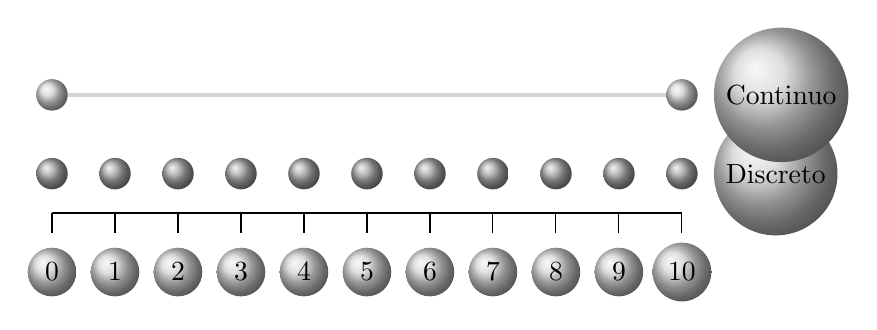
\begin{tikzpicture}[xscale=0.8]
    \definecolor{darkgray}{rgb}{0.66, 0.66, 0.66};
    \definecolor{lightgray}{rgb}{0.83, 0.83, 0.83};
%    \definecolor{firebrick2}{RGB}{205,38,38};
%    \definecolor{royalblue2}{RGB}{67,110,238};
\node [anchor=west] at (10.5,1.25) {Discreto};
\node [anchor=west] at (10.5,2.25) {Continuo};
\foreach \n in {0,...,10} {
    \node at (\n,0) {\n};
    \draw (\n,0.5)--(\n,0.75);
  }
 \tikzstyle{every node}=[draw=none,shape=circle,ball color=darkgray,minimum size=4mm];
\foreach \n in {0,...,10} {
    \node at (\n,1.25) {};
}
\draw (0,0.75) --(10,0.75);
 \tikzstyle{every node}=[draw=none,shape=circle,ball color=lightgray,minimum size=4mm];
\node (r1) at (0,2.25) {};
\node  (r10)  at (10,2.25) {};
\draw [color=lightgray,ultra thick] (r1.east)--(r10.west);
\end{tikzpicture}
\caption{Le variabili continue possono assumere un insieme continuo di valori, al contrario delle variabili discrete, per le quali l'insieme dei possibili valori ha cardinalità al più numerabile.}
\label{fig:DiscreteContinuous}
\end{figure}

Quando una variabile può assumere qualsiasi valore entro un intervallo specificato, allora si dice che la variabile è continua. 
%Una variabile continua può assumere qualsiasi valore all'interno di un intervallo specificato. 
In teoria, ciò significa che frazioni e decimali possono essere utilizzati per raggiungere un livello di precisione qualsiasi. 
In pratica, a un certo punto dobbiamo arrotondare i numeri, rendendo tecnicamente la variabile discreta. 
In variabili veramente discrete, tuttavia, non è possibile aumentare a piacimento il livello di precisione della misurazione.

\section{Perché certe misure sono migliori di altre?}

In psicologia, ciò che vogliamo misurare non è una caratteristica fisica, ma invece è un concetto teorico inosservabile, ovvero un costrutto. 
Ad esempio, supponiamo che un docente voglia valutare quanto bene uno studente comprenda la distinzione tra le quattro diverse scale di misura che sono state descritte sopra. 
Il docente potrebbe predisporre un test costituito da un insieme di domande e potrebbe contare a quante domande lo studente risponde correttamente. 
Questo test, però, può o può non essere una buona misura del costrutto relativo alla conoscenza effettiva delle quattro scale di misura. 
Per esempio, se il docente scrive le domande del test in modo ambiguo o se usa una linguaggio troppo tecnico che lo studente non conosce, allora i risultati del test potrebbero suggerire che lo studente non conosce la materia in questione anche se in realtà questo non è vero. 
D'altra parte, se il docente prepara un test a scelta multipla con risposte errate molto ovvie, allora lo studente può ottenere dei buoni risultati al test anche senza essere in grado di comprendere adeguatamente le proprietà delle quattro scale di misura.

In generale non è possibile misurare un costrutto senza una certa quantità di errore.
Poniamoci dunque il problema di determinare in che modo una misurazione possa dirsi adeguata. 


\subsection{Tipologie di errori}
\label{sec:accuratezza_precisione}

L'errore  è,  per  definizione,  la  differenza  tra  il  valore  vero  e  il  valore misurato della grandezza in esame.  
Gli errori sono classificati  come  sistematici  (o  determinati) e  casuali  (o indeterminati). 
Gli errori casuali sono fluttuazioni, in eccesso o in difetto rispetto al  valore  reale,  delle  singole  determinazioni  e  sono  dovuti  alle molte variabili  incontrollabili che  influenzano  ogni  misura  psicologica.  
Gli errori sistematici, invece, influiscono sulla misurazione sempre nello stesso senso e, solitamente, per una stessa quantità (possono essere additivi o proporzionali). 

Le differenze tra le due tipologie di errori, sistematici e casuali, introducono i concetti di accuratezza e di precisione della misura. 
Una misura viene definita:
\begin{itemize}
\item \emph{accurata}, quando vi è un accordo tra la misura effettuata ed il valore reale;
\item \emph{precisa} quando, ripetendo più volte la misura, i risultati ottenuti sono  concordanti, cioè differiscono in maniera irrilevante tra loro.
\end{itemize}
La metafora del tiro a bersaglio (Figura~\ref{fig:precisione_accuratezza}) illustra la relazione tra precisione e accuratezza.

\begin{figure}
\centering

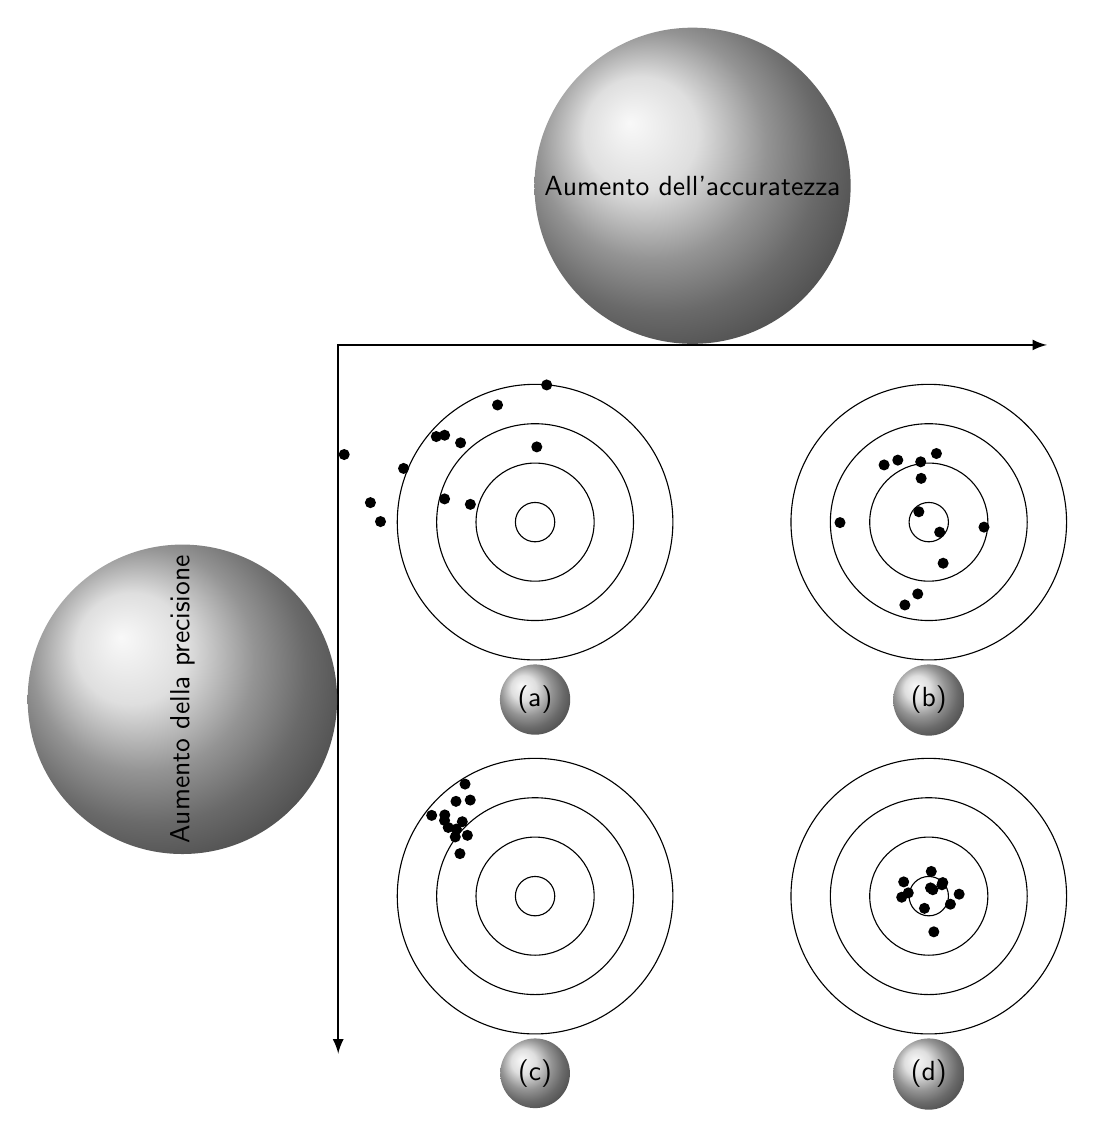
\begin{tikzpicture}[font=\sffamily]

\draw[latex-latex,thick](0,-9) -- node[midway,sloped,above] {Aumento della  precisione}
(0,0) -- node[midway,sloped,above] {Aumento dell'accuratezza} (9,0);
%
\begin{scope}[shift={(2.5,-2.25)}]
 \foreach \X in {0.25,0.75,1.25,1.75}
 {\draw (0,0) circle (\X);}
 \node[anchor=north] at (-90:1.8) {(a)};
 \foreach \X in {1,...,12}
  \fill (-1,1) + (rand*360:rand*1.5) circle(2pt);
\end{scope}
%
\begin{scope}[shift={(7.5,-2.25)}]
 \foreach \X in {0.25,0.75,1.25,1.75}
 {\draw (0,0) circle (\X);}
 \node[anchor=north] at (-90:1.8) {(b)};
 \foreach \X in {1,...,12}
  \fill  (rand*360:rand*1.5) circle(2pt);
\end{scope}
%
\begin{scope}[shift={(2.5,-7)}]
 \foreach \X in {0.25,0.75,1.25,1.75}
 {\draw (0,0) circle (\X);}
 \node[anchor=north] at (-90:1.8) {(c)};
 \foreach \X in {1,...,12}
  \fill (-1,1) + (rand*360:rand*0.5) circle(2pt);
\end{scope}
%
\begin{scope}[shift={(7.5,-7)}]
 \foreach \X in {0.25,0.75,1.25,1.75}
 {\draw (0,0) circle (\X);}
 \node[anchor=north] at (-90:1.8) {(d)};
 \foreach \X in {1,...,12}
  \fill  (rand*360:rand*0.5) circle(2pt);
\end{scope}
\end{tikzpicture}

\caption{Illustrazione dei concetti di precisione e accuratezza: (a) bassa precisione e bassa accuratezza, (b) bassa precisione e alta accuratezza, (c) alta precisione e bassa accuratezza, (d) alta precisione e alta accuratezza.}
    \label{fig:precisione_accuratezza}
\end{figure}

Per tenere sotto controllo l'incidenza degli errori, sono stati introdotti in psicologia i concetti di attendibilità e validità:
\begin{itemize}
\item l'\emph{attendibilità} esprime il grado  di  accordo  o  coerenza  tra misurazioni indipendenti dello stesso costrutto psicologico\footnote{Un costrutto rappresenta il risultato di una fondata riflessione scientifica, non è per definizione accessibile all'osservazione diretta, ma viene inferito dall'osservazione di opportuni indicatori (Sartori, 2005).};
\item la \emph{validità} descrive il grado  in  cui  uno  strumento  misura  ciò che dice di misurare.
\end{itemize}


\subsection{Attendibilità}
\label{sec:reliability}

Uno strumento si dice attendibile quando valuta in modo coerente e stabile la stessa variabile: i risultati ottenuti si mantengono costanti dopo ripetute somministrazione ed in assenza di variazioni psicologiche e fisiche dei soggetti sottoposti al test o cambiamenti dell'ambiente in cui ha luogo la somministrazione. 


\subsection{Validità}
\label{sec:validity}

L'attendibilità di uno strumento non è sufficiente: 
in primo luogo uno strumento di misura deve essere valido, laddove la validità rappresenta il grado in cui uno strumento misura effettivamente ciò che dovrebbe misurare. 
In genere, si fa riferimento ad almeno quattro tipi di validità.
\begin{itemize}
\item La \emph{validità di costrutto} riguarda il grado in cui un test misura ciò per cui è stato costruito.  
Essa si suddivide in: validità convergente e validità divergente. 
La validità convergente fa riferimento alla concordanza tra uno strumento e un altro che misura lo stesso costrutto. 
La validità divergente, al contrario, valuta il grado di discriminazione tra strumenti che misurano costrutti differenti. 
Senza validità di costrutto le  altre forme di validità non hanno senso. 

\item In base alla \emph{validità di contenuto}, un test fornisce una misura valida di un attributo psicologico se il dominio dell'attributo è rappresentato in maniera adeguata dagli item del test. 
Un requisito di base della validità di contenuto è  la rilevanza e la rappresentatività del contenuto degli item in  riferimento all'attributo che il test intende misurare. 

\item La \emph{validità di criterio} valuta il grado di concordanza tra i risultati dello strumento considerato e i risultati ottenuti da altri strumenti che misurano lo stesso costrutto, o tra i risultati dello strumento considerato e un criterio esterno. Nella validità concorrente, costrutto e criterio vengono misurati contestualmente, consentendo un confronto immediato. Nella validità predittiva, il costrutto viene misurato prima e il criterio in un momento successivo, consentendo la valutazione della capacità dello strumento di predire un evento futuro.

\item Infine, la \emph{validità di facciata} fa riferimento al grado in cui il test appare valido ai soggetti a cui esso è diretto. La validità di facciata è importante in ambiti particolari, quali ad esempio la selezione del personale per una determinata occupazione. In questo caso è ovviamente importante che chi si sottopone al test ritenga che il test vada a misurare quegli aspetti che sono importanti per le mansioni lavorative che dovranno essere svolte, piuttosto che altre cose. In generale, la validità di facciata non è utile, tranne in casi particolari.
\end{itemize}


\section*{Conclusioni}

Una domanda che uno psicologo spesso si pone è: ``sulla base delle evidenze  osservate, possiamo concludere dicendo che l'intervento psicologico è efficace nel trattamento e nella cura del disturbo?'' Le considerazioni svolte in questo capitolo dovrebbero farci capire che, prima di cercare di rispondere a questa domanda con l'analisi statistica dei dati, devono essere affrontati i problemi della validità e dell'attendibilità delle misure (oltre a stabilire l'appropriato livello di scala di misura delle osservazioni). L'attendibilità è un prerequisito della validità. Se gli errori di misurazione sono troppo grandi, i dati sono inutili.  Inoltre, uno strumento di misurazione può essere preciso ma non valido. La validità e l'attendibilità delle misurazioni sono dunque entrambe necessarie. 

In generale,  l'attendibilità e la validità delle misure devono essere valutate per capire se i dati raccolti da un ricercatore siano adeguati (1) per fornire una risposta alla domanda della ricerca, e (2) per giungere alla conclusione proposta dal ricercatore alla luce dei risultati dell'analisi statistica che è stata eseguita. È chiaro che le informazioni fornite in questo capitolo si limitano a scalfire la superficie di questi problemi. I concetti qui introdotti, però, devono sempre essere tenuti a mente e costituiscono il fondamento di quanto verrà esposto nei capitoli successivi.












